\section{Evaluation} \label{sec:evaluation}

We evaluate our system on the multi-class, multi-label detection task as previously described.
Each detection episode takes an image and outputs detections with associated times, based on the order of actions taken.
We evaluate on a popular detection challenge task: the PASCAL VOC 2007 dataset \cite{pascal-voc-2010}.
As shown in \autoref{fig:dataset_stats}, the dataset exhibits a rather modest amount of class co-occurrence.

We learn weights on the training and validation sets, and run our policy on all images in the testing set.
The final evaluation pools all detections up to a certain time, and computes their multi-class AP per image, then averaging over all images.
This is done for different times to plot the AP vs. Time curve over the whole dataset.
The evaluation is slightly different that what is usually done (all detections for a class are pooled across the dataset), but has been used before \cite{Desai2009}.

For the detector actions, we use one-vs-all cascaded deformable part-model detectors on a HOG featurization of the image \cite{Felzenszwalb2010b}, with associated linear classification of the detections.
There are $20$ classes in the PASCAL challenge task, so there are $20$ detector actions.
Running a detector on a PASCAL image takes about $1$ second.
Additionally, we use a classifier from the scene-level GIST feature to class presence, for each class.
This is considered one action, and takes about $0.3$ seconds.

We test three different settings of the start and deadline times.
In the first one, the start time is immediate and execution is cut off at 20 seconds, which is enough time to run basically all actions.
In the second one, execution is cut off after only 10 seconds.
Lastly, we measure performance between 5 seconds and 15 seconds.
These operating points show how our method would behave when deployed in different conditions.

\begin{figure}[h!]
\centering
\subfloat[Occurence of a class with another]{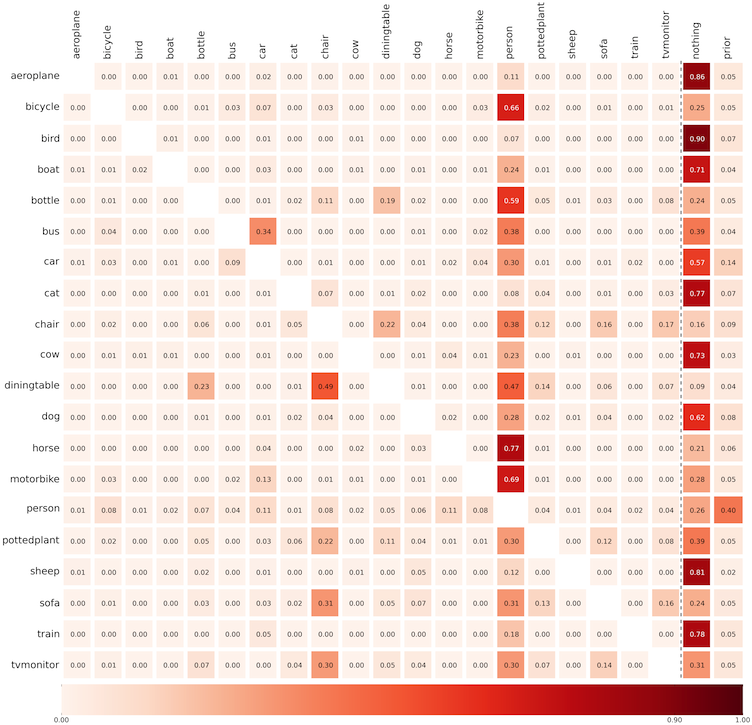
\includegraphics[]
    {../figures/full_pascal_trainval_stats/cooccur_trim.png}} \hfill
\subfloat[Occurence of a class with two others]{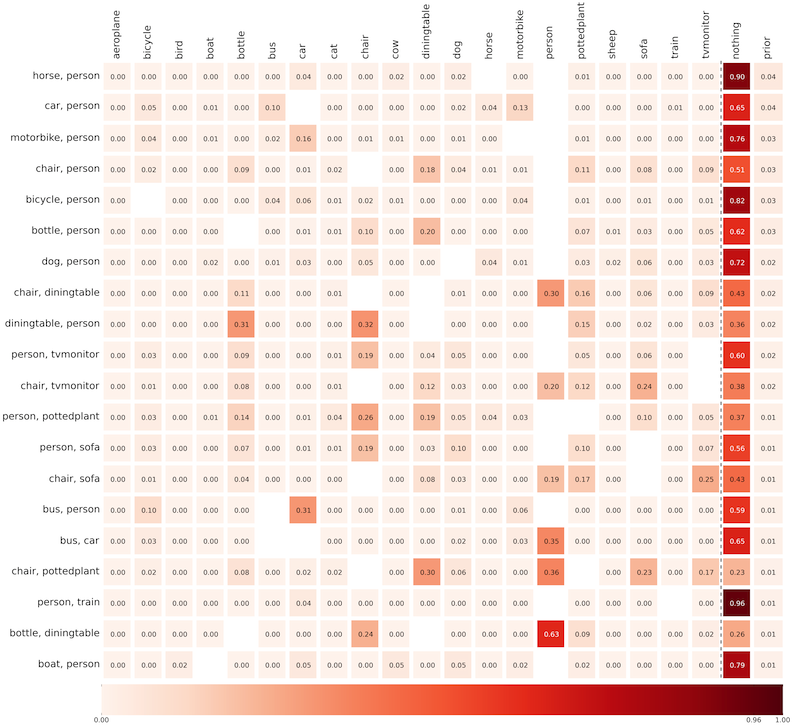
\includegraphics[]
    {../figures/full_pascal_trainval_stats/cooccur_second_order_trim.png}}
  \caption{
  Co-occurrence statistics on the training portion of the PASCAL VOC 2007 dataset.
  In the first plot, a (row,column) cell shows the probability that an image that contains an object of the row class also contains an object of the column class.
  Accordingly, in the second plot, the probability that an image containing objects of the two classes listed in the row also contains an object of the column class.
  }
  \label{fig:dataset_stats}
\end{figure}

\begin{figure}[h!]
\centering
\subfloat[AP vs. Time curves for Random, Oracle, the Fixed Order baseline, and our best-performing policy, with start time of 5 seconds and deadline of 15 seconds.]{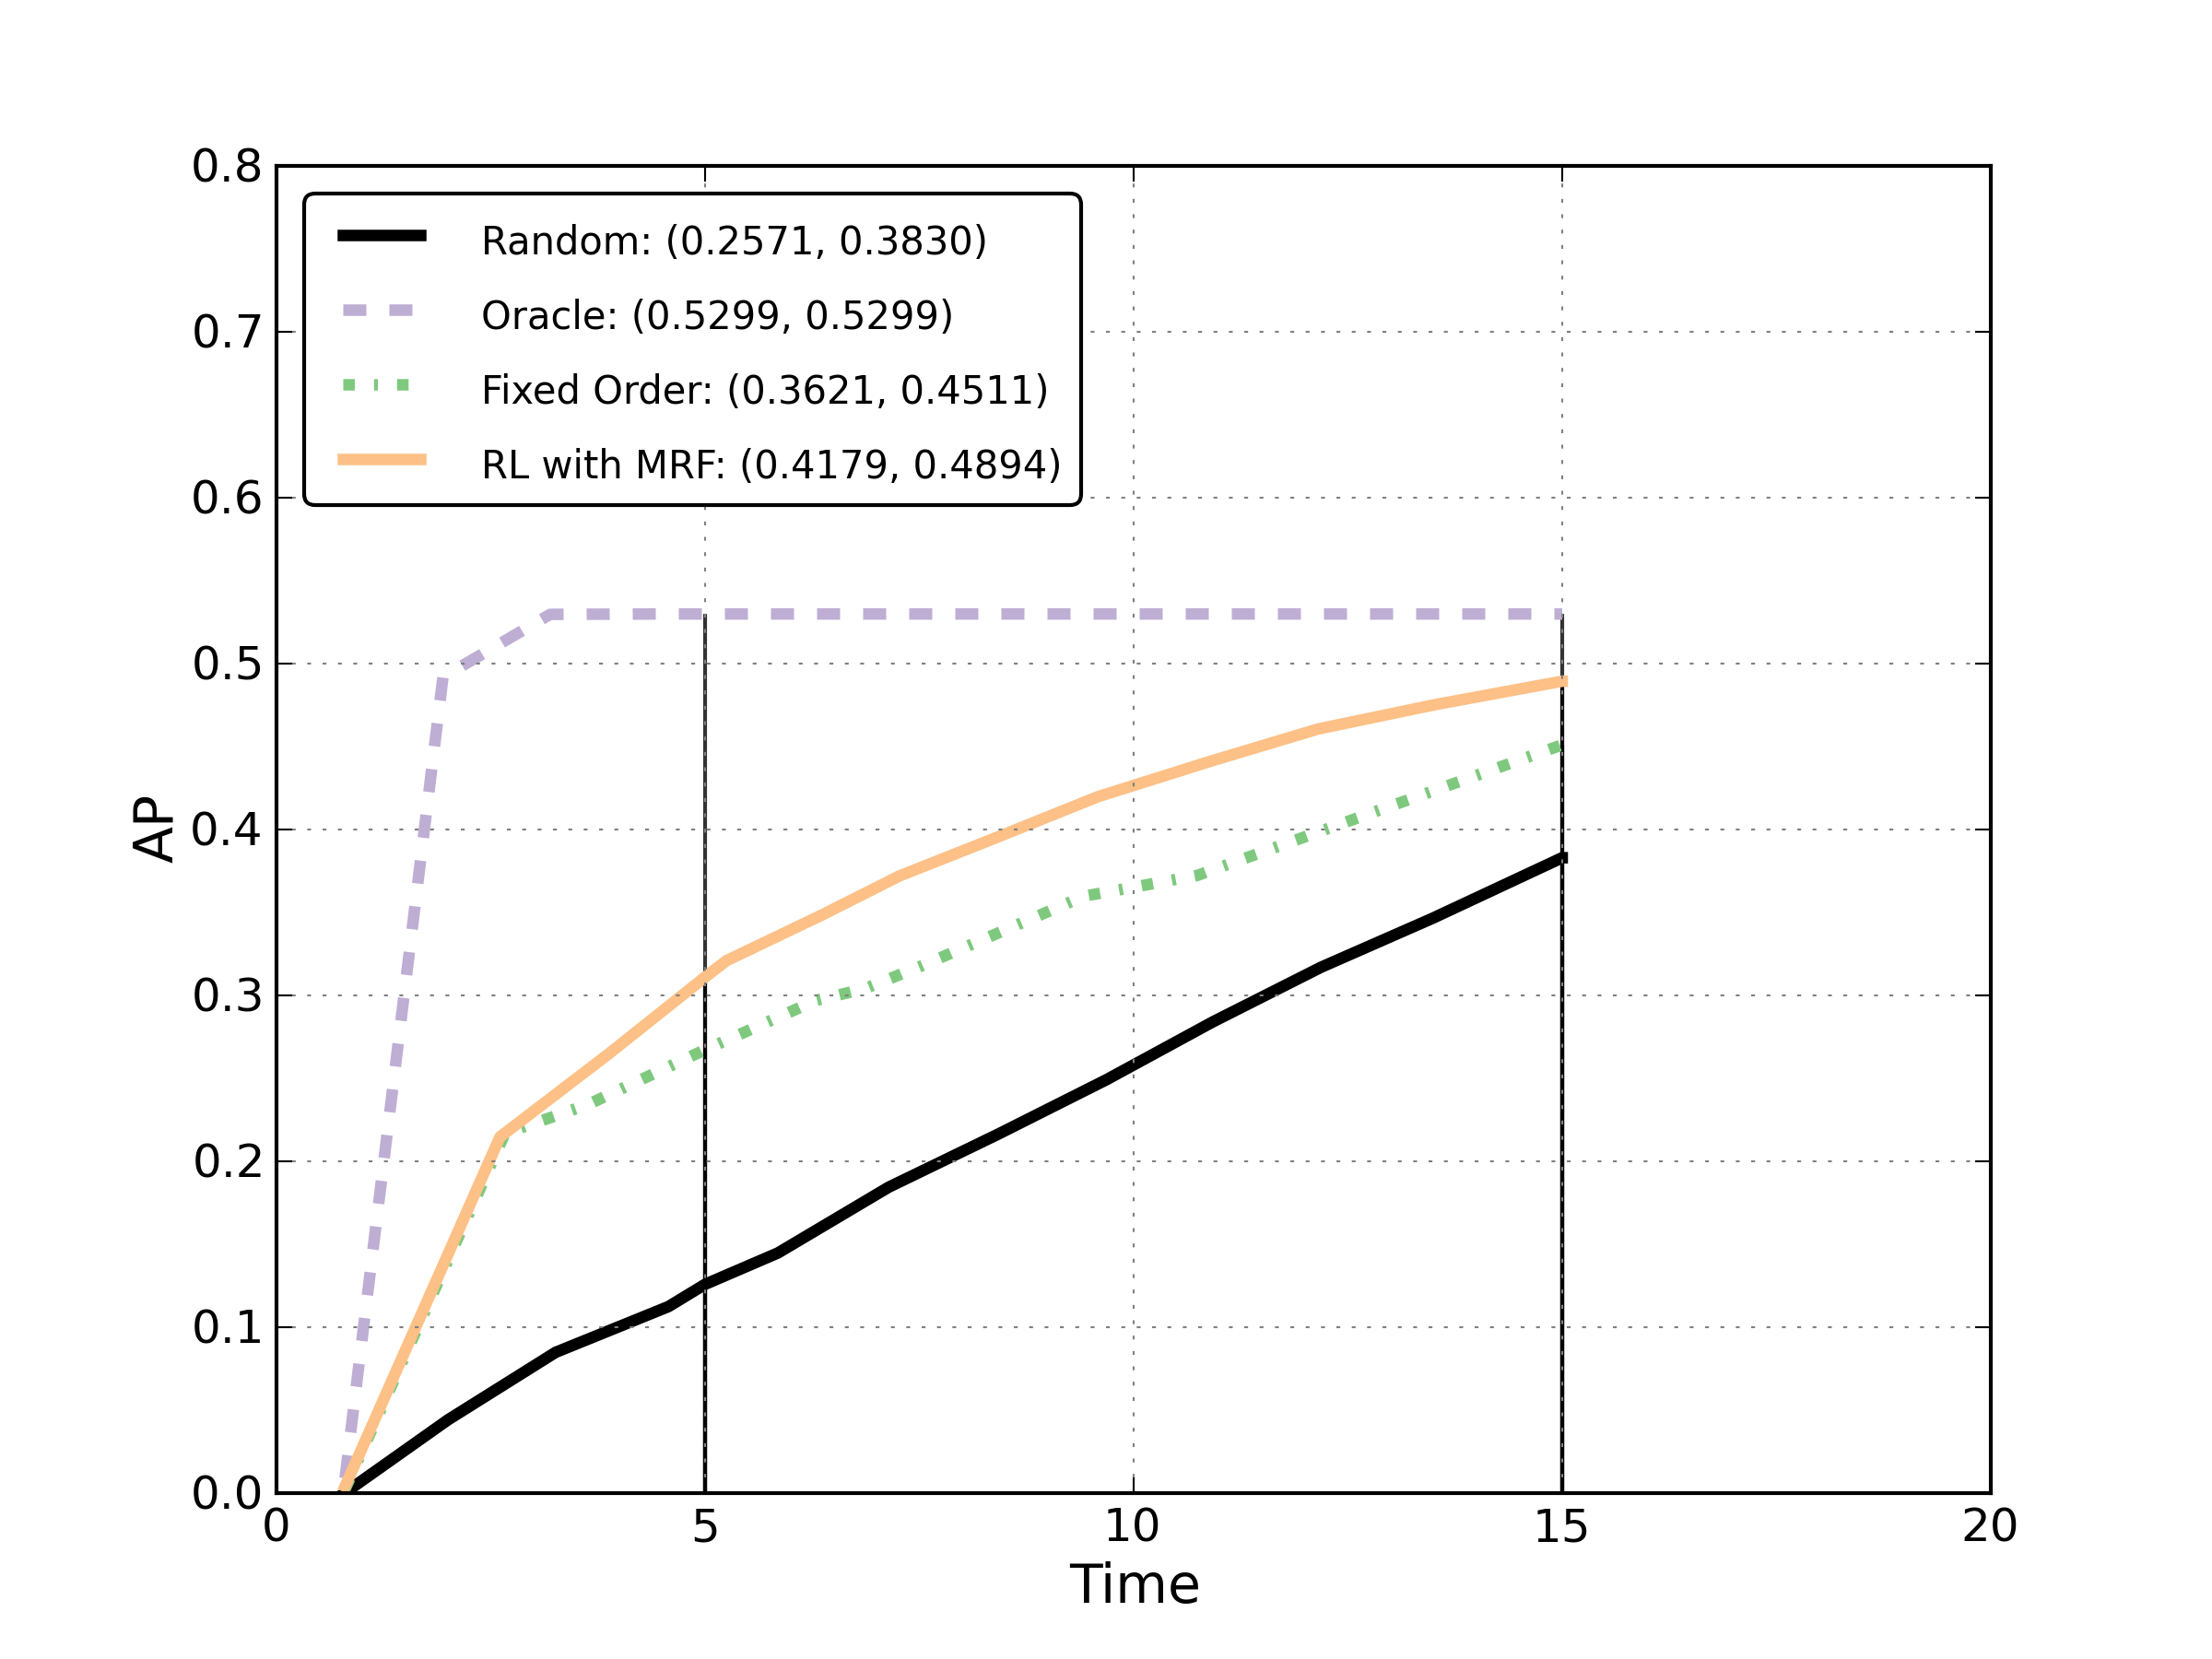
\includegraphics[width=0.47\linewidth]
    {../figures/final1_515.png}} \hfill
\subfloat[Execution traces of different policies]{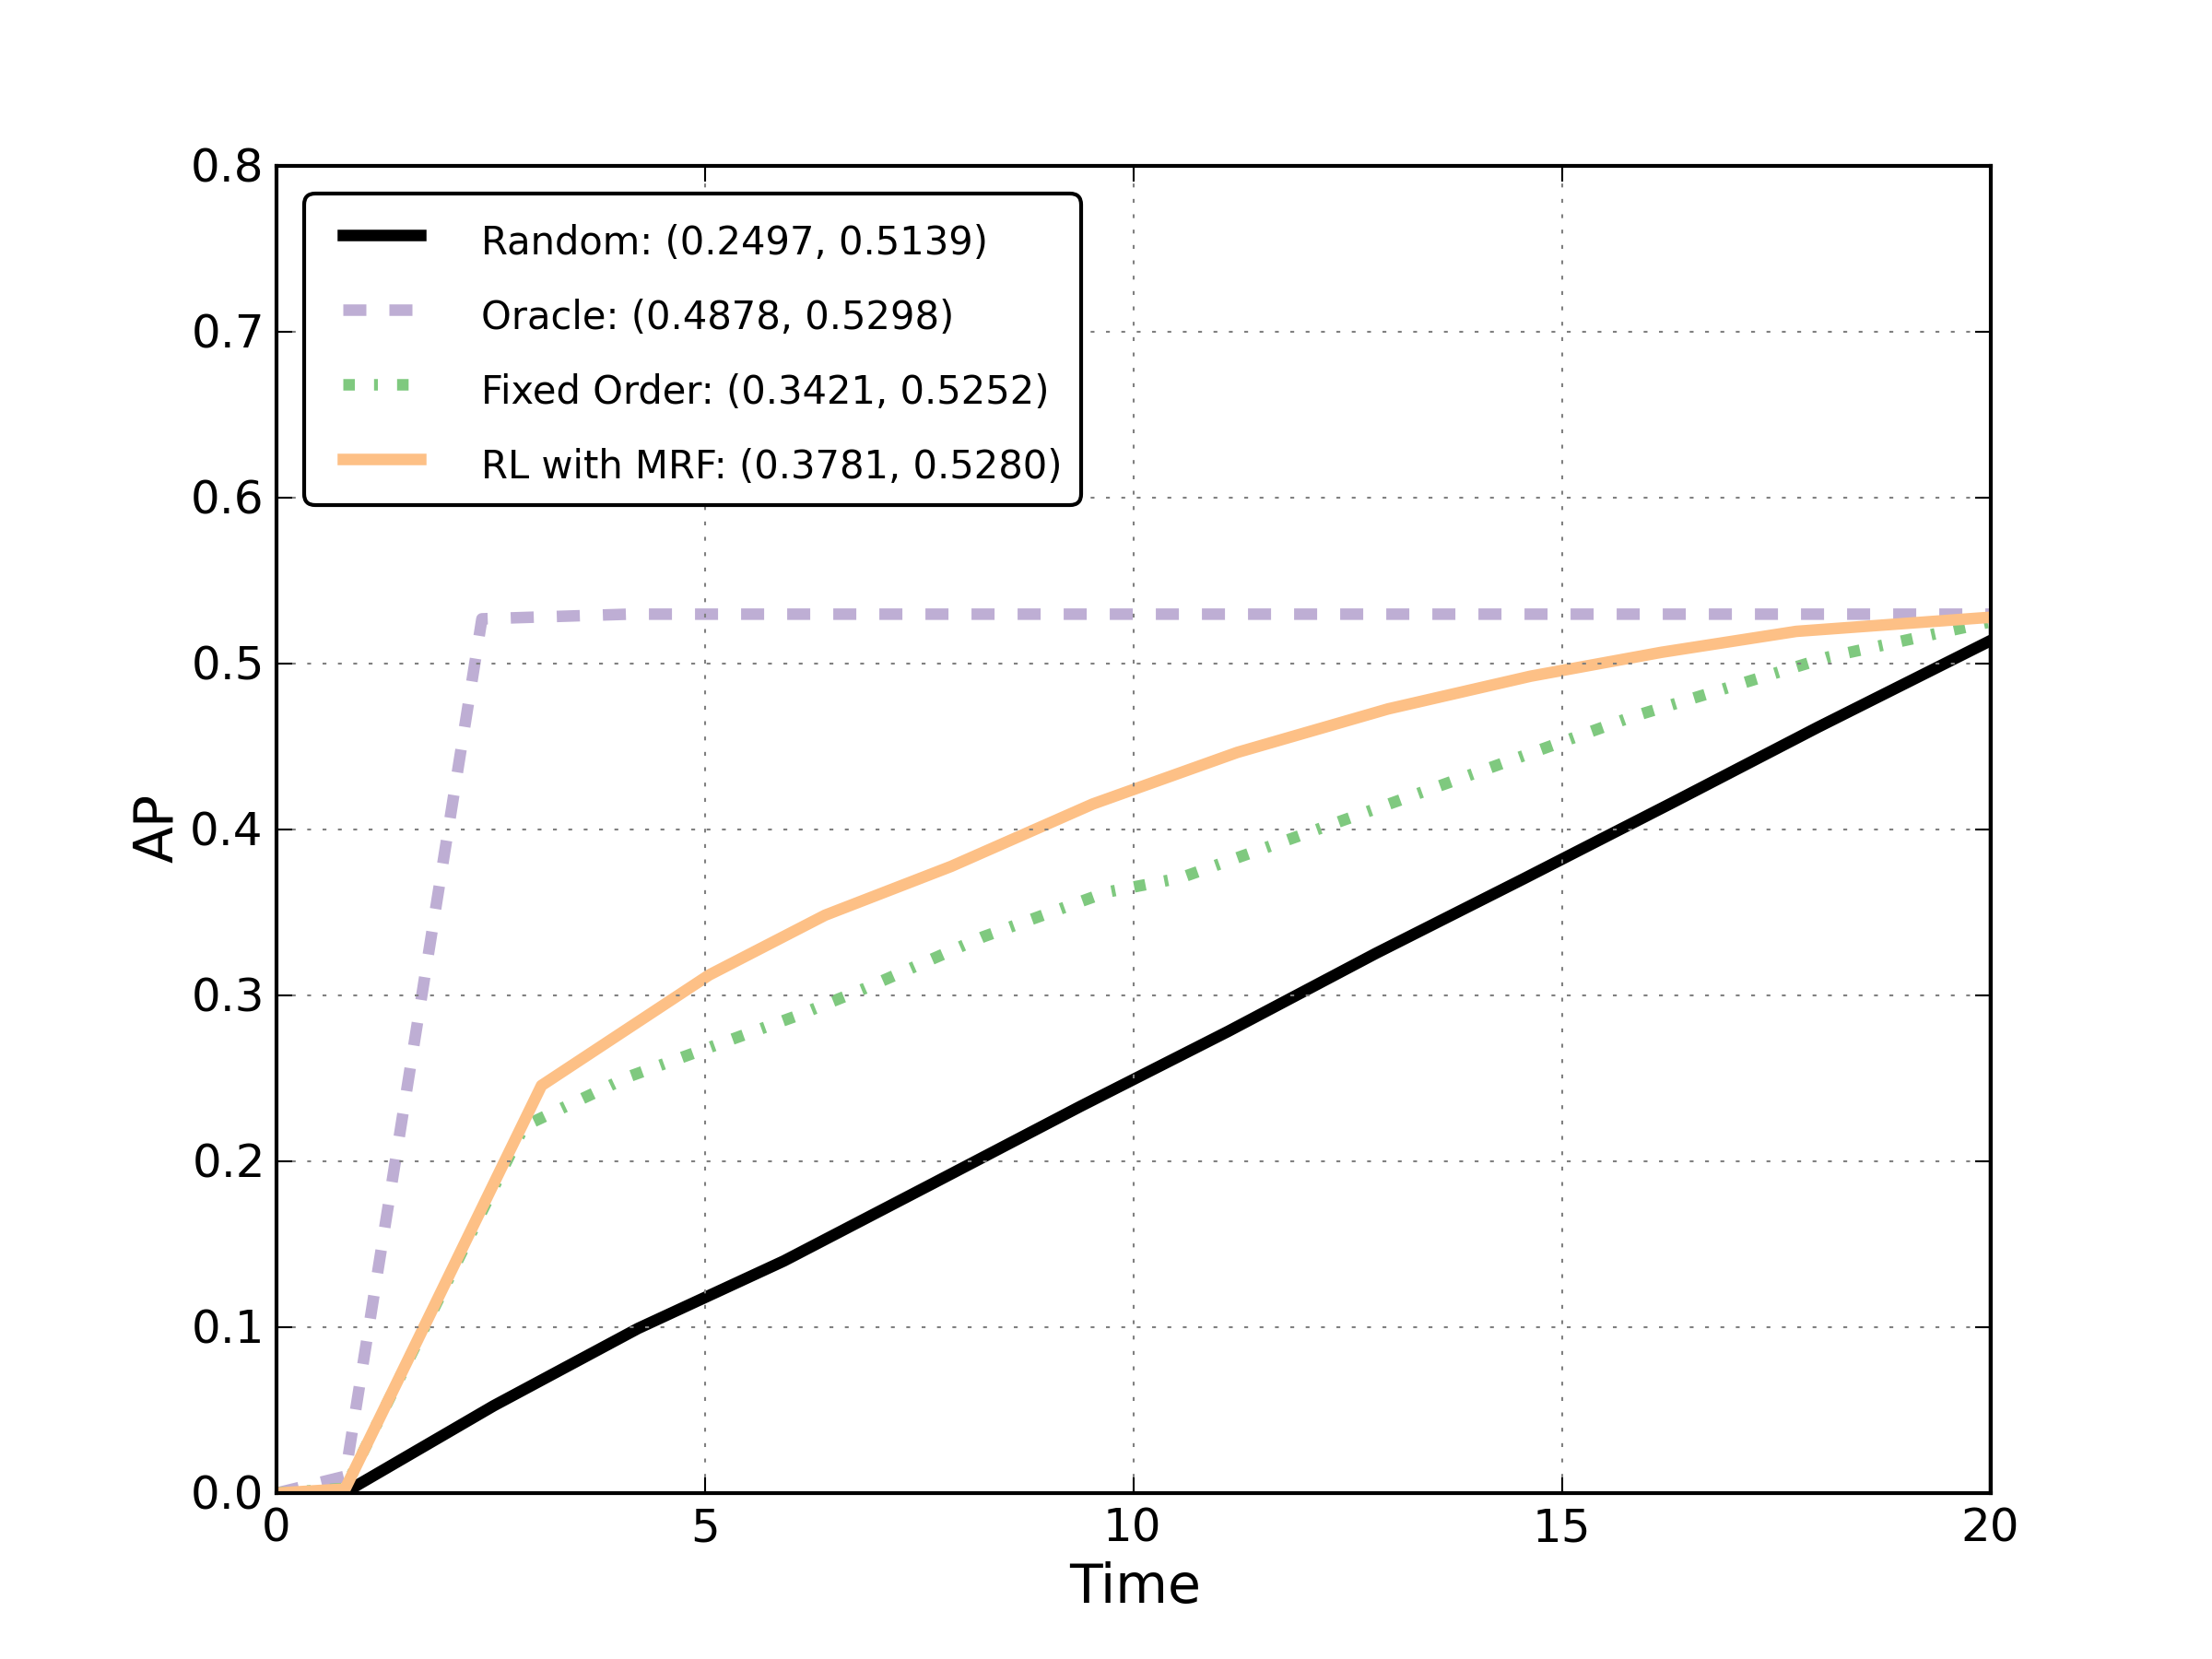
\includegraphics[draft,width=0.47\linewidth]
    {../figures/final1.png}}
  \label{fig:results1}
\end{figure}

We establish the first baseline for our system by selecting actions randomly at each step.
As shown in Figure~\ref{fig:results1}, this \textbf{Random} policy results in a roughly linear gain of AP vs. time.
This is expected: the detectors are capable of obtaining a certain level of performance; if half the detectors are run, the expected performance level is half of the maximum level.

To establish an upper bound on performance, we plot the \textbf{Oracle} policy, obtained by re-ordering the actions with the hindsight of the results they produced.

We consider another baseline: selecting actions in a fixed order based on the value they bring to the AP vs. Time evaluation, which is roughly proportional to their occurrence probability.
We refer to this as \textbf{Fixed Order}.

Then there are our proposed systems, which the previous section thoroughly described: \textbf{RL w/ Direct} and \textbf{RL w/ MRF}.
In experiments, the two were not exceedingly different in performance, with the MRF model consistently performing slightly better.

In \autoref{fig:results1}, we can see that due to the dataset bias, the fixed-order policy performs well at first (as can be seen in \autoref{fig:dataset_stats}, the person class is disproportionately likely to be in the image), but is significantly overtaken by our model as execution goes on.

Lastly, we also evaluate the system that includes a GIST action; this always uses the MRF model to properly update the class probabilities with GIST observations.
This brings another boost in performance.
All results are shown in \autoref{tab:results}.

Additionally, we evaluated different settings of the discount parameter $\gamma$, and found that a mid-range value works best.
We only report results for that value on the test set.
\autoref{fig:weights} shows how changing $\gamma$ affects the learned weights: the GIST action is learned to never be taken in the greedy setting, because it does not nring any immediate detections results.
In the reinforcement learning setting, however (higher $\gamma$), GIST is learned to be taken for its value in quickly refining the class presence probabilities.

\begin{table}[t]
\caption{Results}
\label{tab:results}
\begin{center}
\begin{tabular}{|l|l|l|l|l|l|}
\\ \hline \\
Bounds & Random & Fixed Order & RL w/ MRF & w/ GIST  & Oracle \\ \hline
(0,10) & 0.119  & 0.240       & 0.266     & \textbf{0.267}    & 0.464 \\ 
(0,20) & 0.250  & 0.342       & 0.378     & 0.382    & 0.488 \\ 
(5,15) & 0.257  & 0.362       & 0.418     & 0.420    & 0.530 \\
\end{tabular}
\end{center}
\end{table}

\todo{something about setting values?}
